%!TEX encoding = UTF-8 Unicode
%!TEX root = ../lect-week10.tex

%%%

\ifkompendium\else

\Subsection{Veckans labb: \texttt{maze}}
\begin{Slide}{Veckans labb: \texttt{maze}}\SlideFontSmall
Grunduppgift:
\begin{itemize}
\item Implementera en algoritm som hittar ut ur en labyrint.

\item En labyrint representeras av en \Emph{matris}, \\närmare bestämt en \Emph{vektor av vektorer} med  \Alert{booelska} värden: \\ \code{Vector[Vector[Boolean]]} 

\pause Där de två olika sanningsvärdena representerar följande:
\begin{itemize}\SlideFontSmall
\item \code{true} om det \Emph{finns en vägg} på en viss plats i matrisen
\item \code{false} om det \Alert{inte} finns en vägg på en viss plats i matrisen 

\end{itemize}
\pause
\item Använd enkel idé (som inte ger kortaste vägen): \\ Behåll vänster hand i kontakt med väggen och gå tills du når utgången.

\item Vad krävs av labyrinten för att detta ska fungera?  
\end{itemize}
\pause Extrauppgift:
\begin{itemize}
\item Generera slumpmässig labyrint 
\item Algoritmen (\emph{Prims algoritm}) är given i pseudokod
\end{itemize}

\end{Slide}

\begin{Slide}{Labyrint som booelsk matris}
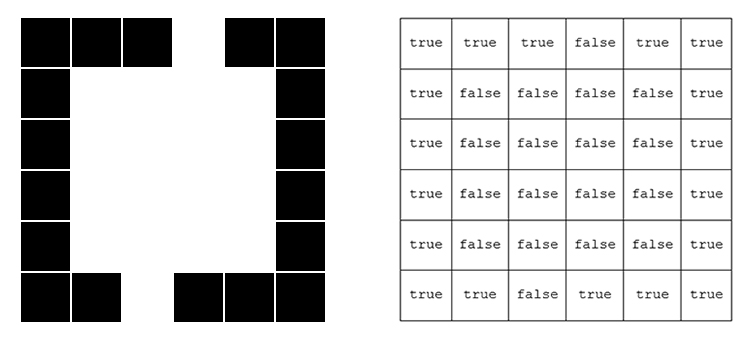
\includegraphics[width=1.0\textwidth]{../img/w09-lab/MazeAndMatrix.jpg}
\end{Slide}

\Subsection{Matriser}

\begin{Slide}{Vad är en matris?}\SlideFontSmall
\begin{multicols}{2}
\begin{itemize}
\item En \Emph{matris} inom \Alert{matematiken} innehåller \Emph{rader} med lika många tal och \Emph{kolumner} med lika många tal. 

\item En matris av dimension $m\times{}n$ har $m \cdot n$ stycken element. 

\end{itemize}

\columnbreak
\begin{itemize}
\item En matris $M_{2,5}$ ritas inom matematiken ofta så här:
\end{itemize}
\[
M=
  \begin{pmatrix}
    5 & 2 & 42 & 4 & 5 \\
    3 & 4 & 18 & 6 & 7
  \end{pmatrix}
\]

\begin{itemize}
\pause
\item Indexering inom matematiken sker från 1 (men oftast från 0 i datorprogram).

\item Vad har talet 42 för index i matrisen M ovan?
\end{itemize}
\end{multicols}
\end{Slide}

\begin{Slide}{En matris med vektorer av vektorer}
Inom programmering används ordet \Emph{matris} ofta för att beteckna en \Alert{nästlade struktur} i två dimensioner, till exempel en instans av typen \code{Array[Array[Int]]}
\begin{REPL}
scala> val xss = Array(Array(5,2,42,4,5),Array(3,4,18,6,7))
xss: Array[Array[Int]] = Array(Array(5, 2, 42, 4, 5), Array(3, 4, 18, 6, 7))
\end{REPL}
\pause
Man indexerar i en nästlad sekvens med upprepad \code{apply}:
\begin{REPL}
scala> xss(0)(2)
res0: ???                   // Vad är typ och värde?

scala> xss.apply(0).apply(2)
res1: ???                   // Vad är typ och värde?

scala> xss(0)
res2: ???                   // Vad är typ och värde?
\end{REPL}

\end{Slide}

\begin{Slide}{En matris med vektorer av vektorer}
Inom programmering används ordet \Emph{matris} ofta för att beteckna en \Alert{nästlade struktur} i två dimensioner, till exempel en instans av typen \code{Array[Array[Int]]}
\begin{REPL}
scala> val xss = Array(Array(5,2,42,4,5),Array(3,4,18,6,7))
xss: Array[Array[Int]] = Array(Array(5, 2, 42, 4, 5), Array(3, 4, 18, 6, 7))
\end{REPL}

Man indexerar i en nästlad sekvens med upprepad \code{apply}:
\begin{REPL}
scala> xss(0)(2)
res0: Int = 42

scala> xss.apply(0).apply(2)
res1: Int = 42

scala> xss(0)
res2: Array[Int] = Array(5, 2, 42, 4, 5)
\end{REPL}
\end{Slide}

\begin{Slide}{Uppdatering av en förändringsbar nästlad struktur}
Man kan förändra en array av arrayer ''på plats'' med tilldelning:
\begin{REPL}
scala> val xss = Array(Array(5,2,42,4,5),Array(3,4,18,6,7))

scala> xss(0)(0) = 100

scala> xss
res0: ???

scala> xss(0)(2) = xss(0)(2) - 1

scala> xss
res1: ???

scala> xss(1) = Array.fill(5)(-1)

scala> xss
res2: ???
\end{REPL}
\end{Slide}

\begin{Slide}{Uppdatering av en förändringsbar nästlad struktur}
Man kan förändra en array av arrayer ''på plats'' med tilldelning:
\begin{REPL}
scala> val xss = Array(Array(5,2,42,4,5),Array(3,4,18,6,7))

scala> xss(0)(0) = 100

scala> xss
res0: Array[Array[Int]]=Array(Array(100, 2, 42, 4, 5), Array(3, 4, 18, 6, 7))

scala> xss(0)(2) = xss(0)(2) - 1

scala> xss
res1: Array[Array[Int]]=Array(Array(100, 2, 41, 4, 5), Array(3, 4, 18, 6, 7))

scala> xss(1) = Array.fill(5)(-1)

scala> xss
res2: Array[Array[Int]]=Array(Array(100, 2, 41, 4, 5), Array(-1,-1,-1,-1,-1))
\end{REPL}
\end{Slide}

\begin{Slide}{Olika sätt att skapa förändringsbara matriser}\SlideFontSmall
Det jobbiga, primitiva sättet:
\begin{REPL}
scala> val xs = new Array[Array[Int]](2)
xs: Array[Array[Int]] = Array(null, null)

scala> for (i <- xs.indices) {xs(i) = new Array[Int](5)}

scala> xs
res0: Array[Array[Int]] = Array(Array(0, 0, 0, 0, 0), Array(0, 0, 0, 0, 0))

scala> println(xs)
[[I@196a99d0
\end{REPL}
Enklare sätt:
\begin{REPL}
scala> val xs = Array.ofDim[Int](2,5)
xs: Array[Array[Int]] = Array(Array(0, 0, 0, 0, 0), Array(0, 0, 0, 0, 0))
\end{REPL}
Enklare och tydligare sätt, där initialvärdet anges explicit:
\begin{REPL}
scala> Array.fill(2,5)(0)
res37: Array[Array[Int]] = Array(Array(0, 0, 0, 0, 0), Array(0, 0, 0, 0, 0))
\end{REPL}

\end{Slide}

\begin{Slide}{Skapa oföränderlig nästlad struktur}
\begin{REPL}
scala> Vector.fill(2,5)(0)

scala> Vector.tabulate(5,2)((x,y) => x + y + 1)
res0: 
  scala.collection.immutable.Vector[scala.collection.immutable.Vector[Int]] = 
  Vector(Vector(1,2), Vector(2,3), Vector(3,4), Vector(4,5), Vector(5,6))


\end{REPL}

\end{Slide}

\begin{Slide}{Uppdatering av en oföränderlig nästlad struktur}
\end{Slide}


\begin{Slide}{Iterering över nästlad struktur}
\end{Slide}


\begin{Slide}{Matris som Array med Array med heltal i Java}
\begin{Code}[language=Java]
public class ArrayMatrix {

    public static void showMatrix(int[][] m){
        System.out.println("\n--- showMatrix ---");
        for (int row = 0; row < m.length; row++){
            for (int col = 0; col < m[row].length; col++) {
                System.out.print("[" + row + "]");
                System.out.print("[" + col + "] = ");
                System.out.print(m[row][col] + "; ");
            }
            System.out.println();
        }
    }
    
    public static void main(String[] args) {
        int[][] xss = new int[10][5];
        showMatrix(xss);
    }
}
\end{Code}
\end{Slide}

\fi











